\documentclass[border=3pt]{standalone}
\usepackage[utf8]{inputenc}
\usepackage[T1]{fontenc}
\usepackage{lmodern}
\renewcommand{\familydefault}{\sfdefault}
\usepackage{sansmath}\sansmath
\usepackage{chemfig}
\usepackage{pgfplots}\pgfplotsset{compat=1.18,/pgf/number format/use comma,/pgf/number format/1000 sep={.}}
\usetikzlibrary{arrows.meta,calc,positioning,decorations.pathmorphing,patterns}
% paleta del sitio
\definecolor{nar}{HTML}{E8680C}\definecolor{narc}{HTML}{FFB35C}\definecolor{hielo}{HTML}{FFF3E8}
\definecolor{tinta}{HTML}{1D1D1F}\definecolor{gris}{HTML}{6E6E73}\definecolor{lila}{HTML}{7C5CF0}
\definecolor{azul}{HTML}{2F6FD6}\definecolor{menta}{HTML}{17A673}\definecolor{coral}{HTML}{E8342A}
\setchemfig{atom sep=2em,bond style={line width=0.8pt}}
\tikzset{lab/.style={font=\small\bfseries,text=nar},pie/.style={font=\footnotesize,text=tinta,align=center}}
\begin{document}
\scalebox{0.85}{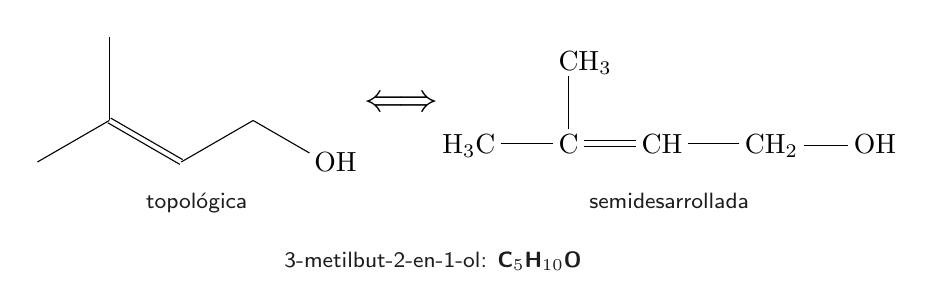
\begin{tikzpicture}
\node at (0,0) {\chemfig{-[:30](-[:90])=[:-30]-[:30]-[:-30]OH}};
\node at (2.6,0) {\Large $\Longleftrightarrow$};
\node at (6.0,0) {\chemfig{H_3C-C(-[2]CH_3)=CH-CH_2-OH}};
\node[pie,anchor=north] at (0,-1.0) {topológica};
\node[pie,anchor=north] at (6.0,-1.0) {semidesarrollada};
\node[pie] at (3,-2.0) {3-metilbut-2-en-1-ol: \textbf{C$_5$H$_{10}$O}};
\end{tikzpicture}}
\end{document}
